\documentclass[border=5pt]{standalone}
\usepackage[T1]{fontenc}
\usepackage{lmodern}
\usepackage{pgfplots}
\usepgfplotslibrary{groupplots}
\pgfplotsset{compat=1.18}
\begin{document}\sffamily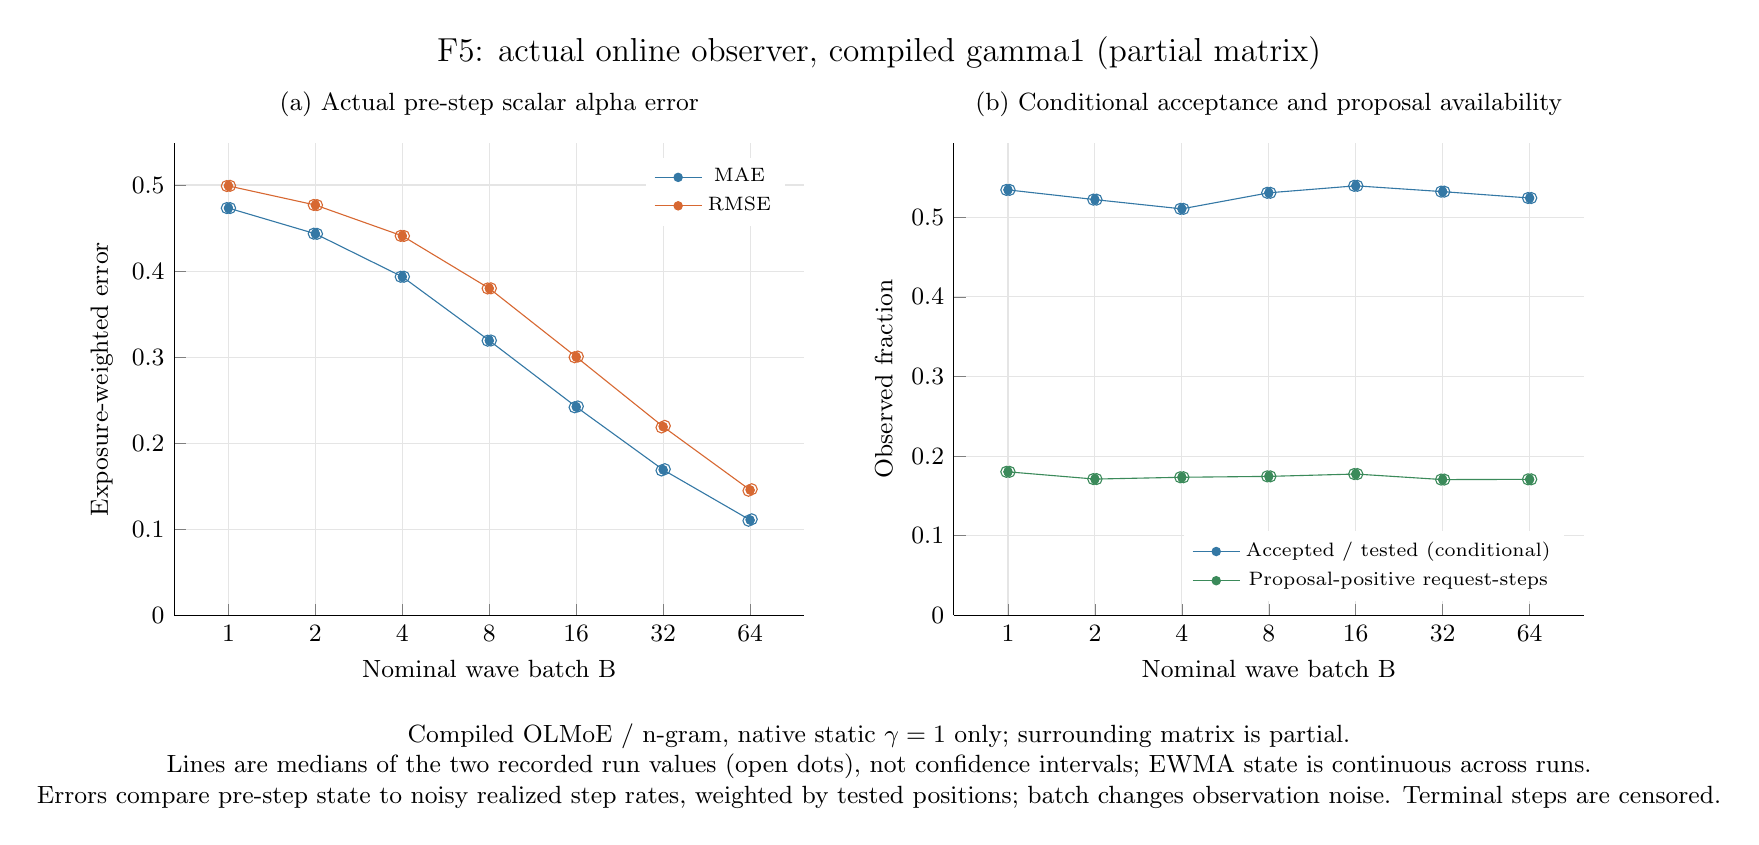
\begin{tikzpicture}
\definecolor{cal}{HTML}{3478A5}\definecolor{test}{HTML}{D76832}\definecolor{profile}{HTML}{3B8A5A}
\begin{groupplot}[group style={group size=2 by 1,horizontal sep=1.9cm},width=8.0cm,height=6.0cm,scale only axis,axis lines*=left,grid=major,grid style={gray!20},tick label style={font=\small},label style={font=\small},title style={font=\small},legend style={font=\scriptsize,draw=none},unbounded coords=jump]
\nextgroupplot[title={(a) Actual pre-step scalar alpha error},ylabel={Exposure-weighted error},xmode=log,log basis x=2,xtick={1,2,4,8,16,32,64},xticklabels={1,2,4,8,16,32,64},xlabel={Nominal wave batch B},ymin=0,legend pos=north east]\addplot[color=cal,mark=*,mark size=1.5pt] coordinates {(1,0.473223159184) (2,0.44336839148) (4,0.393423865496) (8,0.319249232268) (16,0.242226312074) (32,0.169070568433) (64,0.110738591686)};
\addlegendentry{MAE}
\addplot[forget plot,only marks,color=cal,mark=o,mark size=2.0pt,mark options={fill=white}] coordinates {(0.987,0.473233180343) (1.974,0.443473018344) (3.948,0.393406755364) (7.896,0.319146029062) (15.792,0.241705941426) (31.584,0.168328428915) (63.168,0.109895589718) (64.832,0.111581593653) (32.416,0.169812707951) (16.208,0.242746682723) (8.104,0.319352435475) (4.052,0.393440975629) (2.026,0.443263764616) (1.013,0.473213138025)};
\addplot[color=test,mark=*,mark size=1.5pt] coordinates {(1,0.498964146442) (2,0.476764425926) (4,0.440877919175) (8,0.379905713912) (16,0.300274532572) (32,0.219208607798) (64,0.145629037927)};
\addlegendentry{RMSE}
\addplot[forget plot,only marks,color=test,mark=o,mark size=2.0pt,mark options={fill=white}] coordinates {(0.987,0.498841186632) (1.974,0.476855636363) (3.948,0.440926393473) (7.896,0.379845295793) (15.792,0.299875699219) (31.584,0.218287656954) (63.168,0.144741776625) (64.832,0.146516299228) (32.416,0.220129558642) (16.208,0.300673365925) (8.104,0.379966132031) (4.052,0.440829444877) (2.026,0.476673215489) (1.013,0.499087106252)};
\nextgroupplot[title={(b) Conditional acceptance and proposal availability},ylabel={Observed fraction},xmode=log,log basis x=2,xtick={1,2,4,8,16,32,64},xticklabels={1,2,4,8,16,32,64},xlabel={Nominal wave batch B},ymin=0,legend pos=north east,legend pos=south east]\addplot[color=cal,mark=*,mark size=1.5pt] coordinates {(1,0.534339622642) (2,0.522116903633) (4,0.510522213562) (8,0.530691530692) (16,0.539463601533) (32,0.532168387609) (64,0.52414885194)};
\addlegendentry{Accepted / tested (conditional)}
\addplot[forget plot,only marks,color=cal,mark=o,mark size=2.0pt,mark options={fill=white}] coordinates {(0.987,0.534339622642) (1.974,0.522116903633) (3.948,0.510522213562) (7.896,0.530691530692) (15.792,0.539463601533) (31.584,0.532168387609) (63.168,0.52414885194) (64.832,0.52414885194) (32.416,0.532168387609) (16.208,0.539463601533) (8.104,0.530691530692) (4.052,0.510522213562) (2.026,0.522116903633) (1.013,0.534339622642)};
\addplot[color=profile,mark=*,mark size=1.5pt] coordinates {(1,0.180223068553) (2,0.171127331711) (4,0.173401811056) (8,0.174508474576) (16,0.17745444656) (32,0.17048070413) (64,0.170767982693)};
\addlegendentry{Proposal-positive request-steps}
\addplot[forget plot,only marks,color=profile,mark=o,mark size=2.0pt,mark options={fill=white}] coordinates {(0.987,0.180223068553) (1.974,0.171127331711) (3.948,0.173401811056) (7.896,0.174508474576) (15.792,0.17745444656) (31.584,0.17048070413) (63.168,0.170767982693) (64.832,0.170767982693) (32.416,0.17048070413) (16.208,0.17745444656) (8.104,0.174508474576) (4.052,0.173401811056) (2.026,0.171127331711) (1.013,0.180223068553)};
\end{groupplot}
\path (group c1r1.north west) -- node[above=0.8cm,font=\large] {F5: actual online observer, compiled gamma1 (partial matrix)} (group c2r1.north east);
\path (group c1r1.south west) -- node[below=1.25cm,align=center,font=\small] {Compiled OLMoE / n-gram, native static $\gamma=1$ only; surrounding matrix is partial.\\Lines are medians of the two recorded run values (open dots), not confidence intervals; EWMA state is continuous across runs.\\Errors compare pre-step state to noisy realized step rates, weighted by tested positions; batch changes observation noise. Terminal steps are censored.} (group c2r1.south east);
\end{tikzpicture}\end{document}
